% Options for packages loaded elsewhere
\PassOptionsToPackage{unicode}{hyperref}
\PassOptionsToPackage{hyphens}{url}
\PassOptionsToPackage{dvipsnames,svgnames,x11names}{xcolor}
\documentclass[
]{article}
\usepackage{xcolor}
\usepackage[margin=2.5cm]{geometry}
\usepackage{amsmath,amssymb}
\setcounter{secnumdepth}{-\maxdimen} % remove section numbering
\usepackage{iftex}
\ifPDFTeX
  \usepackage[T1]{fontenc}
  \usepackage[utf8]{inputenc}
  \usepackage{textcomp} % provide euro and other symbols
\else % if luatex or xetex
  \usepackage{unicode-math} % this also loads fontspec
  \defaultfontfeatures{Scale=MatchLowercase}
  \defaultfontfeatures[\rmfamily]{Ligatures=TeX,Scale=1}
\fi
\usepackage{lmodern}
\ifPDFTeX\else
  % xetex/luatex font selection
\fi
% Use upquote if available, for straight quotes in verbatim environments
\IfFileExists{upquote.sty}{\usepackage{upquote}}{}
\IfFileExists{microtype.sty}{% use microtype if available
  \usepackage[]{microtype}
  \UseMicrotypeSet[protrusion]{basicmath} % disable protrusion for tt fonts
}{}
\makeatletter
\@ifundefined{KOMAClassName}{% if non-KOMA class
  \IfFileExists{parskip.sty}{%
    \usepackage{parskip}
  }{% else
    \setlength{\parindent}{0pt}
    \setlength{\parskip}{6pt plus 2pt minus 1pt}}
}{% if KOMA class
  \KOMAoptions{parskip=half}}
\makeatother
\usepackage{longtable,booktabs,array}
\usepackage{calc} % for calculating minipage widths
% Correct order of tables after \paragraph or \subparagraph
\usepackage{etoolbox}
\makeatletter
\patchcmd\longtable{\par}{\if@noskipsec\mbox{}\fi\par}{}{}
\makeatother
% Allow footnotes in longtable head/foot
\IfFileExists{footnotehyper.sty}{\usepackage{footnotehyper}}{\usepackage{footnote}}
\makesavenoteenv{longtable}
\usepackage{graphicx}
\makeatletter
\newsavebox\pandoc@box
\newcommand*\pandocbounded[1]{% scales image to fit in text height/width
  \sbox\pandoc@box{#1}%
  \Gscale@div\@tempa{\textheight}{\dimexpr\ht\pandoc@box+\dp\pandoc@box\relax}%
  \Gscale@div\@tempb{\linewidth}{\wd\pandoc@box}%
  \ifdim\@tempb\p@<\@tempa\p@\let\@tempa\@tempb\fi% select the smaller of both
  \ifdim\@tempa\p@<\p@\scalebox{\@tempa}{\usebox\pandoc@box}%
  \else\usebox{\pandoc@box}%
  \fi%
}
% Set default figure placement to htbp
\def\fps@figure{htbp}
\makeatother
\usepackage{svg}
\ifLuaTeX
\usepackage[bidi=basic]{babel}
\else
\usepackage[bidi=default]{babel}
\fi
\babelprovide[main,import]{english}
% get rid of language-specific shorthands (see #6817):
\let\LanguageShortHands\languageshorthands
\def\languageshorthands#1{}
\ifLuaTeX
  \usepackage[english]{selnolig} % disable illegal ligatures
\fi
\setlength{\emergencystretch}{3em} % prevent overfull lines
\providecommand{\tightlist}{%
  \setlength{\itemsep}{0pt}\setlength{\parskip}{0pt}}
\usepackage[]{biblatex}
\addbibresource{../references.bib}
\usepackage{bookmark}
\IfFileExists{xurl.sty}{\usepackage{xurl}}{} % add URL line breaks if available
\urlstyle{same}
\hypersetup{
  pdftitle={The Automatic Statistician, revisited},
  pdfauthor={Warith Harchaoui},
  pdflang={en},
  colorlinks=true,
  linkcolor={Maroon},
  filecolor={Maroon},
  citecolor={Blue},
  urlcolor={Blue},
  pdfcreator={LaTeX via pandoc}}

\title{The Automatic Statistician, revisited}
\usepackage{etoolbox}
\makeatletter
\providecommand{\subtitle}[1]{% add subtitle to \maketitle
  \apptocmd{\@title}{\par {\large #1 \par}}{}{}
}
\makeatother
\subtitle{A technical report on the repository}
\author{Warith Harchaoui}
\date{9 November 2026}

\begin{document}
\maketitle

\begin{figure}
\centering
\pandocbounded{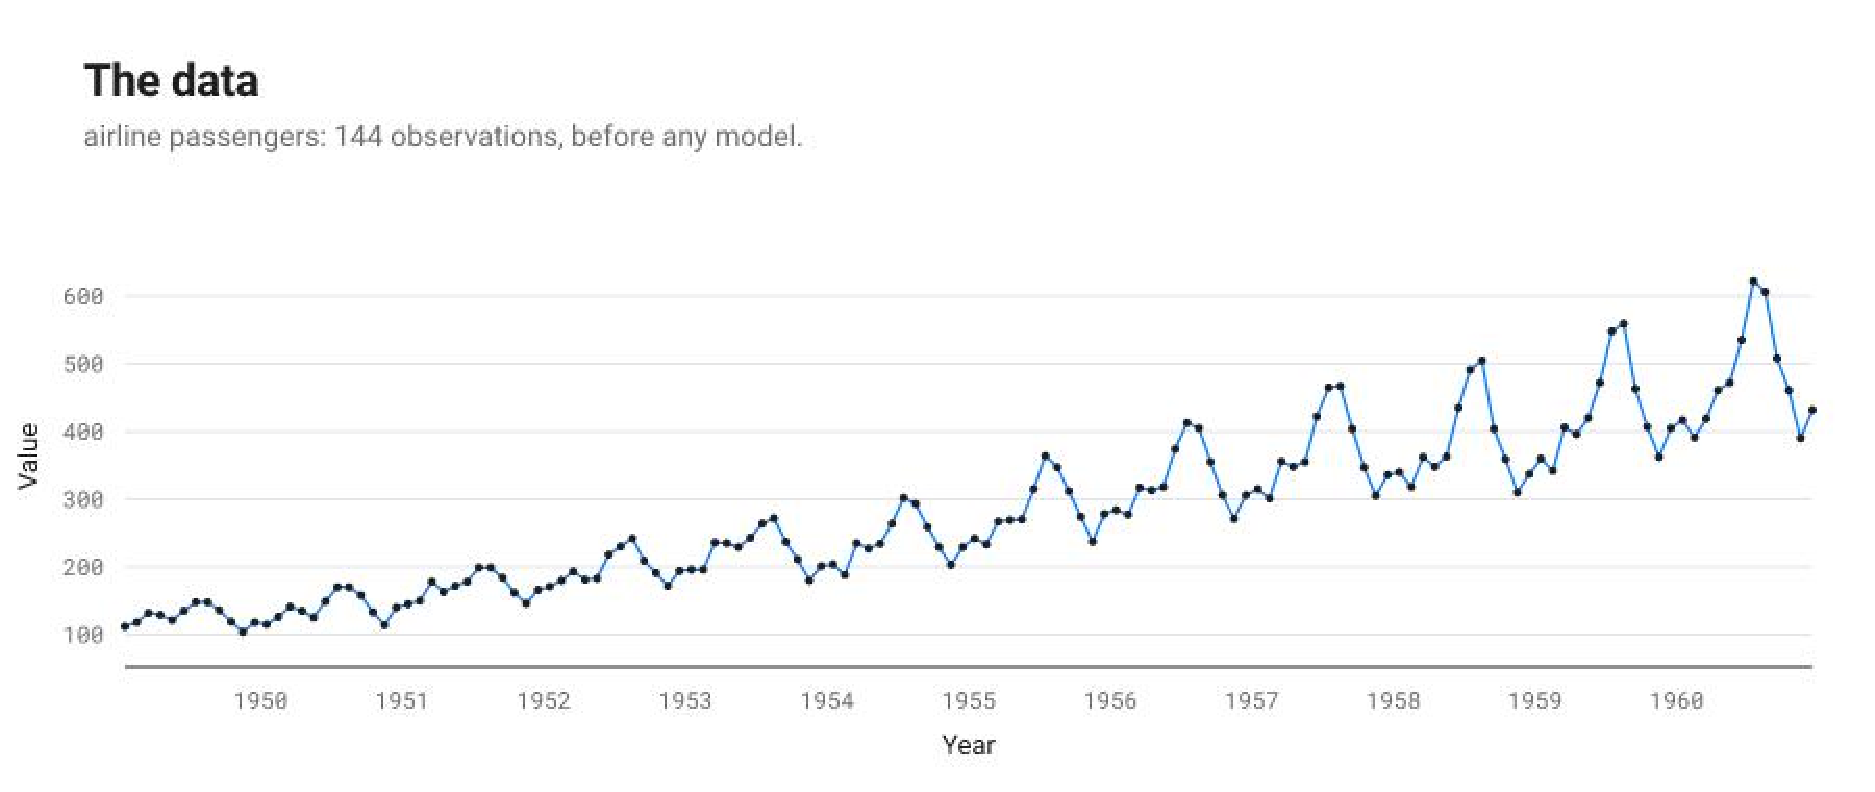
\includegraphics[keepaspectratio]{../figures/data_airline.pdf}}
\caption{Monthly airline passengers from 1949 to 1960, in thousands.
This series runs through the whole report, as it ran through the 2014
paper.}
\end{figure}

\section{Summary}\label{summary}

In 2014 a program read twelve years of airline passengers and wrote, in
plain English, that the series holds a linear trend, a yearly cycle
whose amplitude grows with the trend and noise that grows too. Nobody
told it to look for a year. That program was the Automatic Statistician
\autocite{duvenaud2013cks,lloyd2014abcd}, written in Python 2.7 and
MATLAB.

This repository brings it back to life in Python 3 with \texttt{torch}.
It also ports AutoGP \autocite{saad2023autogp} from Julia and runs the
2014 extrapolation benchmark again, this time against the forecasting
methods of 2026.

The program works in four steps:

\begin{enumerate}
\def\labelenumi{\arabic{enumi}.}
\tightlist
\item
  Given a time series, the structure search looks for the expression
  over Gaussian-process kernels that explains the data best by the
  Bayesian information criterion (BIC) \autocite{schwarz1978bic}.
\item
  The search splits that expression into additive components and
  describes each one in English.
\item
  Each component is checked against its prior
  \autocite{lloyd2015criticism}.
\item
  A report gathers everything. It now writes the expression as a formula
  with its fitted parameters. It also says how much the data prefer the
  kept structure to the next one.
\end{enumerate}

The main results:

\begin{itemize}
\tightlist
\item
  \textbf{The port is faithful.} The 2014 system published 130 models
  (13 series, 10 search levels each). All 130 reproduce their negative
  log likelihood: twelve series to within \(5\times10^{-5}\) nats, the
  ill-conditioned solar series to within \(5\times10^{-3}\). The
  component sentences of the airline report match the original word for
  word. Two series have been searched again from scratch so far. On
  both, the ten-level search reaches a BIC at least as good as the
  published one (lower is better): airline 1108.9 against 1123.7, solar
  −872.3 against −870.3.
\item
  \textbf{AutoGP agrees with its original.} Every deterministic quantity
  of the port matches AutoGP.jl to \(10^{-12}\) or better. The
  comparison also turned up a surprise: the Hamiltonian moves of
  AutoGP.jl see only the gradient of the prior.
\item
  \textbf{The 2014 forecasts hold up in 2026.} On the thirteen series,
  24 methods are compared by mean standardised error. The published ABCD
  forecasts come fifth by mean (2.05), behind three pre-trained
  foundation models and N-BEATS
  \autocite{ansari2025chronos2,mistral2026timestral,amazon2024chronosbolt,oreshkin2020nbeats}.
  They never fail badly: the worst series scores 4.00. Eureqa
  \autocite{schmidt2009distilling}, the symbolic-regression baseline of
  2014, has a comparable median (2.82). Its mean climbs to 48.11 because
  of one series, where its formula extrapolates 590 times worse than the
  best method. PySR \autocite{cranmer2023pysr}, run here on the same
  split, stays bounded on that series (4.56) and has a mean of 2.76.
\item
  \textbf{The structure search is a symbolic regression.} Its grammar
  builds kernel expressions where symbolic regression builds arithmetic
  ones. The reports now state the formula found. The section ``What the
  formula contains'' shows what that formula holds and what it leaves
  out. Eureqa, PySR and their successors read more easily. The structure
  search models noise and uncertainty. It also extrapolates somewhat
  better than PySR here. On smooth components, their formulas and ours
  complement each other.
\end{itemize}

\section{The system}\label{the-system}

\subsection{What the search looks for}\label{what-the-search-looks-for}

A Gaussian process (GP) \autocite{rasmussen2006gpml} is a probability
distribution over functions. With a zero mean, as here, the covariance
\(k(t, t')\) fixes it. It says how strongly the values at times \(t\)
and \(t'\) move together. The search builds covariances from base
kernels:

\begin{longtable}[]{@{}
  >{\raggedright\arraybackslash}p{(\linewidth - 4\tabcolsep) * \real{0.3333}}
  >{\raggedright\arraybackslash}p{(\linewidth - 4\tabcolsep) * \real{0.3333}}
  >{\raggedright\arraybackslash}p{(\linewidth - 4\tabcolsep) * \real{0.3333}}@{}}
\toprule\noalign{}
\begin{minipage}[b]{\linewidth}\raggedright
symbol
\end{minipage} & \begin{minipage}[b]{\linewidth}\raggedright
base kernel
\end{minipage} & \begin{minipage}[b]{\linewidth}\raggedright
what it describes
\end{minipage} \\
\midrule\noalign{}
\endhead
\bottomrule\noalign{}
\endlastfoot
\texttt{SE} & squared exponential & a smooth function \\
\texttt{Per} & periodic & a repeating pattern, with its period \\
\texttt{Lin} & linear & a linear trend (products of them make
polynomials) \\
\texttt{C} & constant & an offset \\
\texttt{WN} & white noise & uncorrelated noise \\
\texttt{RQ} & rational quadratic (2013 grammar only) & smoothness at
several scales \\
\end{longtable}

Operators combine them. A sum adds independent components. A product
modulates one component by another: \texttt{Lin\ x\ Per} is a cycle
whose amplitude grows linearly. Two operators of the 2014 grammar switch
between regimes: the changepoint \texttt{CP} and the change window
\texttt{CW}.

One level of the search runs as follows:

\begin{enumerate}
\def\labelenumi{\arabic{enumi}.}
\tightlist
\item
  The grammar rewrites one subexpression of each current expression at a
  time. The rewrites are the candidates.
\item
  Each candidate's parameters are fitted by maximising the GP marginal
  likelihood (L-BFGS here, conjugate gradients in GPML
  \autocite{rasmussen2010gpmltoolbox}).
\item
  The candidates are ranked by BIC. The best few seed the next level.
\end{enumerate}

The 2014 configuration searches ten levels.

\subsection{From expression to report}\label{from-expression-to-report}

The winning kernel is rewritten as a sum of products. Each product is
one additive component. The components are ordered by how much each one
lowers the cross-validated mean absolute error of extrapolation. The
original's rule system then describes each one: ``An approximately
periodic function with a period of 1.0 years and with linearly
increasing amplitude.''

Model checking compares each component's posterior with its prior
through four statistics: quantiles, autocorrelation, periodogram and
maximum mean discrepancy
\autocite{gretton2012kernel,lloyd2015criticism}. The report comes in two
formats, as the 2014 system wrote it. md2star compiles the Markdown
version to PDF and \texttt{latexmk} compiles the LaTeX version.
Sprezzature-figures draws the figures.

\subsection{AutoGP: a posterior over
structures}\label{autogp-a-posterior-over-structures}

AutoGP \autocite{saad2023autogp} grew out of Bayesian synthesis of
probabilistic programs \autocite{saad2019bayesian}. It replaces the
greedy search by sequential Monte Carlo. The data enter in batches. A
population of structures is reweighted by how well each one predicted
the batch, then resampled, then moved by structure proposals and by
Hamiltonian Monte Carlo on the parameters. The result is a weighted
posterior over structures. Their forecasts are averaged.
\texttt{autostat.smc} ports AutoGP.jl \autocite{saad2023autogpjl}. Each
heavy structure of its posterior gets the 2014 report and its checks.

\subsection{Surfaces}\label{surfaces}

The same service layer answers from six places:

\begin{itemize}
\tightlist
\item
  a Python library
\item
  a command line written with Click
\item
  a local GUI generated by sprezzature-cli-gui
\item
  an HTTP API written with FastAPI
\item
  an MCP server (FastAPI-MCP, four tools)
\item
  an Agent Skill, routed by \texttt{TRIGGERS.md}
\end{itemize}

\section{How faithful the port is}\label{how-faithful-the-port-is}

The port keeps what decides the results: the original's
parameterisation, grammar, simplification rules, initialisation
heuristics, BIC parameter count and greedy loop (\texttt{PORTING.md}).
It changes three things. The optimiser is L-BFGS. The covariances are
written in \texttt{torch}, where autograd replaces hand-written
derivatives. The parallelism is new. \texttt{PORTING.md} also documents
four defects found in the original. None of them changes a published
number.

\begin{longtable}[]{@{}
  >{\raggedright\arraybackslash}p{(\linewidth - 2\tabcolsep) * \real{0.5000}}
  >{\raggedright\arraybackslash}p{(\linewidth - 2\tabcolsep) * \real{0.5000}}@{}}
\toprule\noalign{}
\begin{minipage}[b]{\linewidth}\raggedright
check
\end{minipage} & \begin{minipage}[b]{\linewidth}\raggedright
result
\end{minipage} \\
\midrule\noalign{}
\endhead
\bottomrule\noalign{}
\endlastfoot
NLL of the 130 published models & 12 series within \(5\times10^{-5}\)
nats, solar within \(5\times10^{-3}\) \\
airline component sentences & identical to 2014 \\
gradients against finite differences & within \(10^{-4}\) \\
ten-level search, final BIC (lower is better), two series so far &
airline 1108.9 vs 1123.7, solar −872.3 vs −870.3 \\
\end{longtable}

For AutoGP, \texttt{tests/test\_smc\_julia.py} loads AutoGP.jl v0.1.19
through \texttt{juliacall} and compares the two implementations number
by number:

\begin{itemize}
\tightlist
\item
  the joint densities of 30 structures agree to \(10^{-14}\)
\item
  the covariance matrices agree to \(10^{-15}\)
\item
  the densities of 400 structure moves agree to \(10^{-15}\) and their
  density ratios to \(4\times10^{-13}\)
\item
  the predictive moments agree to \(3\times10^{-12}\)
\end{itemize}

The surprise came from the gradients. On all 359 kernel parameters
tested, the gradient Gen computes equals the gradient of the parameter's
standard normal prior. The reason is that \texttt{covariance\_prior} is
not declared differentiable, so the likelihood never reaches the
leapfrog steps. The Hamiltonian moves of AutoGP.jl explore the prior,
where the intended sampler explores the posterior. The port reproduces
this behaviour by default and offers the intended sampler as
\texttt{HMCConfig(gradient="full")}.

\section{Extrapolation against the methods of
2026}\label{extrapolation-against-the-methods-of-2026}

The 2014 benchmark trains on the first 90 \% of thirteen series and
forecasts the last 10 \%. The repository first recomputes the paper's
table from the published forecasts, to within \(2.2\times10^{-10}\). It
then scores these methods of 2026 on the same split:

\begin{itemize}
\tightlist
\item
  classical models selected by information criterion
  \autocite{hyndman2002ets,hyndman2008forecast,fiorucci2016theta}
\item
  LightGBM \autocite{ke2017lightgbm} and deep networks
  \autocite{oreshkin2020nbeats,challu2023nhits}, tuned by rolling-origin
  cross-validation on the training part only
\item
  pre-trained foundation models, used zero-shot
  \autocite{ansari2024chronos,ansari2025chronos2,das2024timesfm,google2025timesfm25,mistral2026timestral,qu2026kumotabular}.
\end{itemize}

The score is the standardised root mean squared error (RMSE): each
series' error divided by the best error on that series. A score of 1.00
means the method was the best on that series. A score of 2.00 means its
error was twice the best one.

\begin{longtable}[]{@{}
  >{\raggedright\arraybackslash}p{(\linewidth - 8\tabcolsep) * \real{0.2000}}
  >{\raggedright\arraybackslash}p{(\linewidth - 8\tabcolsep) * \real{0.2000}}
  >{\raggedright\arraybackslash}p{(\linewidth - 8\tabcolsep) * \real{0.2000}}
  >{\raggedright\arraybackslash}p{(\linewidth - 8\tabcolsep) * \real{0.2000}}
  >{\raggedright\arraybackslash}p{(\linewidth - 8\tabcolsep) * \real{0.2000}}@{}}
\toprule\noalign{}
\begin{minipage}[b]{\linewidth}\raggedright
method
\end{minipage} & \begin{minipage}[b]{\linewidth}\raggedright
family
\end{minipage} & \begin{minipage}[b]{\linewidth}\raggedright
median
\end{minipage} & \begin{minipage}[b]{\linewidth}\raggedright
mean
\end{minipage} & \begin{minipage}[b]{\linewidth}\raggedright
series won
\end{minipage} \\
\midrule\noalign{}
\endhead
\bottomrule\noalign{}
\endlastfoot
Chronos-2 & foundation & 1.47 & 1.65 & 1 \\
Chronos-Bolt (base) & foundation & 1.53 & 1.70 & 1 \\
Timestral 209M & foundation & 1.57 & 1.65 & 1 \\
KumoTabular on lags & foundation & 1.68 & 2.50 & 2 \\
TimesFM 2.5 & foundation & 1.72 & 2.17 & 0 \\
AutoARIMA & classical & 1.79 & 3.22 & 0 \\
N-HiTS & deep learning & 1.81 & 2.09 & 1 \\
AutoTheta & classical & 1.89 & 2.21 & 0 \\
N-BEATS & deep learning & 1.91 & 1.96 & 0 \\
AutoETS & classical & 1.96 & 2.45 & 0 \\
LightGBM on lags & machine learning & 2.08 & 4.38 & 1 \\
\textbf{ABCD 2014} & structure search & \textbf{2.12} & \textbf{2.05} &
1 \\
Spectral mixture \autocite{wilson2013spectral} & 2014 baseline & 2.19 &
3.22 & 0 \\
\textbf{CKS 2013} & structure search & \textbf{2.48} & \textbf{2.17} &
2 \\
\textbf{Eureqa} \autocite{schmidt2009distilling} & symbolic regression
(2014 published) & \textbf{2.82} & \textbf{48.11} & 1 \\
\textbf{PySR} \autocite{cranmer2023pysr} & symbolic regression &
\textbf{2.87} & \textbf{2.76} & 0 \\
gplearn \autocite{stephens2015gplearn} & symbolic regression & 3.60 &
8.84 & 0 \\
\end{longtable}

The table is abridged from \texttt{benchmark/RESULTS.md}, which lists
all 24 methods. Two readings matter.

First, foundation models, trained on large corpora, now extrapolate
these series best. Chronos-2 has a median standardised error of 1.47 and
ABCD 2.12.

Second, among the methods that fit one model to the series at hand, the
structure search is the most reliable. Its mean (2.05) sits below its
median (2.12), so no series goes badly. Eureqa's mean comes from a
single series, monthly average daily calls, where its formula scores
590.55 against 1.20 for ABCD. Without that series, Eureqa's mean falls
to 2.90.

\section{The structure search as symbolic
regression}\label{the-structure-search-as-symbolic-regression}

\subsection{The parallel}\label{the-parallel}

Symbolic regression \autocite{koza1992genetic} searches a grammar of
expressions, fits each expression's constants and selects by trading
accuracy against complexity. The structure search does the same with
another grammar. Its expressions denote covariances where symbolic
regression's denote regression functions. Marginal likelihood fits its
constants. BIC plays the role of the complexity penalty. Both problems
are NP-hard \autocite{virgolin2022nphard}, so both communities search
heuristically.

\begin{longtable}[]{@{}
  >{\raggedright\arraybackslash}p{(\linewidth - 10\tabcolsep) * \real{0.1667}}
  >{\raggedright\arraybackslash}p{(\linewidth - 10\tabcolsep) * \real{0.1667}}
  >{\raggedright\arraybackslash}p{(\linewidth - 10\tabcolsep) * \real{0.1667}}
  >{\raggedright\arraybackslash}p{(\linewidth - 10\tabcolsep) * \real{0.1667}}
  >{\raggedright\arraybackslash}p{(\linewidth - 10\tabcolsep) * \real{0.1667}}
  >{\raggedright\arraybackslash}p{(\linewidth - 10\tabcolsep) * \real{0.1667}}@{}}
\toprule\noalign{}
\begin{minipage}[b]{\linewidth}\raggedright
method
\end{minipage} & \begin{minipage}[b]{\linewidth}\raggedright
search space
\end{minipage} & \begin{minipage}[b]{\linewidth}\raggedright
search
\end{minipage} & \begin{minipage}[b]{\linewidth}\raggedright
selection
\end{minipage} & \begin{minipage}[b]{\linewidth}\raggedright
output
\end{minipage} & \begin{minipage}[b]{\linewidth}\raggedright
noise
\end{minipage} \\
\midrule\noalign{}
\endhead
\bottomrule\noalign{}
\endlastfoot
Eureqa \autocite{schmidt2009distilling} & arithmetic trees & genetic
programming & accuracy-parsimony front & closed form & implicit \\
PySR \autocite{cranmer2023pysr} & arithmetic trees, user operators &
evolution with annealing & loss-complexity front & closed forms &
implicit, custom loss \\
AI Feynman \autocite{udrescu2020aifeynman,udrescu2020aifeynman2} &
arithmetic, recursively simplified & neural-guided decomposition &
description length & closed form & robust (version 2.0) \\
SINDy \autocite{brunton2016sindy} & span of a fixed library &
thresholded least squares & sparsity & closed-form ODE & smoothing \\
DSR \autocite{petersen2021dsr} & token sequences & policy gradient &
reward & closed form & implicit \\
Transformers \autocite{kamienny2022e2e,biggio2021nesymres} &
pre-training distribution & amortised decoding & fit & closed form & via
training data \\
LLM-SR \autocite{shojaee2025llmsr} & Python programs & proposals from a
language model & fit & program & implicit \\
Bayesian machine scientist \autocite{guimera2020bms} & arithmetic trees
& MCMC & posterior, BIC likelihood & closed forms & Gaussian \\
CKS 2013 \autocite{duvenaud2013cks} & kernel grammar, + and × & greedy
beam & BIC & kernel, GP posterior & Gaussian \\
\textbf{ABCD 2014} \autocite{lloyd2014abcd} & kernel grammar + CP, CW,
WN & greedy beam & BIC & kernel, report, \textbf{formula} & explicit,
heteroscedastic \\
AutoGP \autocite{saad2023autogp} & kernel grammar & SMC & posterior
weight & weighted kernels & Gaussian \\
\end{longtable}

Symbolic-regression benchmarks
\autocite{lacava2021srbench,defranca2025srbenchpp,aldeia2025srbench2,shojaee2025llmsrbench}
measure accuracy and the recovery of known equations on regression
tasks. None of them holds an extrapolation task on real time series, the
very task where the two families differ most.

\subsection{What the formula contains}\label{what-the-formula-contains}

Each report now has a section called ``The formula found''. For the
airline series, the published 2014 model reads

\[y(t) = f_1(t) + f_2(t) + f_3(t) + f_4(t)\]

\[f_1(t) \sim \mathrm{GP}\left(0,\ 1122\,(t - 1946)(t' - 1946)\right),
\qquad f_1(t) = 92.68 + 31.58\,(t - 1949)\]

\[\begin{aligned}
f_2(t) \sim \mathrm{GP}\Big(0,\ & 21.91\,(t - 1945)(t' - 1945) \\
& \cdot \frac{\exp\left(1.924\cos\frac{2\pi (t - t')}{1.002}\right) - I_0(1.924)}{e^{1.924} - I_0(1.924)}
\cdot \exp\left(-\frac{(t - t')^2}{2 \cdot 22.98^2}\right)\Big)
\end{aligned}\]

\[f_3(t) \sim \mathrm{GP}\left(0,\ 0.285\,(t - 1943)(t' - 1943) \cdot \delta_{t t'}\right),
\qquad f_4(t) \sim \mathrm{GP}\left(0,\ 193.1\,\exp\left(-\frac{(t - t')^2}{2 \cdot 0.6787^2}\right)\right)\]

Each line answers a question a statistician would ask:

\begin{itemize}
\tightlist
\item
  The trend \(f_1\) has a closed form, read exactly from its posterior
  mean: 31.6 thousand more passengers each year.
\item
  The cycle \(f_2\) has a period of 1.002 years, with an amplitude that
  grows linearly from 1945. The data found the calendar year to within
  two thousandths of a year, less than a day.
\item
  The noise \(f_3\) grows linearly too.
\item
  The term \(f_4\) is a smooth function with a length scale of 0.68
  years.
\end{itemize}

The solar series gives a more striking result. Its formula shows a
change window \(w_1(t)\) from 1643 to 1716, inside which a constant
\(f(t) = -0.5964\,w_1(t)\) lowers solar irradiance by 0.6 W/m². These
are the years of the Maunder minimum, when sunspots almost vanished.
Nobody told the search about them. It found them!

Every component built from constants and linear kernels gets a closed
form like these, even when a change of regime switches it on or off.
Periodic components get one too, because the periodic kernel is a sum of
cosines:

\[\exp(a\cos u) = I_0(a) + 2\sum_{k \ge 1} I_k(a)\cos(k u).\]

A periodic component's posterior mean is therefore a Fourier series in
the period found. Its weights fall quickly when \(a\) is small. The
report writes the series up to the harmonic after which the rest weighs
less than 0.1 \% of the component and marks it with \(\approx\).

On the thirteen published models this gives a closed form to 16 of the
76 components: trends and offsets, the yearly cycle of the temperature
series (amplitude 4.3 degrees), the weekly and half-yearly cycles of the
births series. Three kinds of component have none: smooth components,
periodic ones modulated by a smooth kernel and noise. A draw from such a
process is no finite formula, so its covariance serves as its formula.
Here the structure search parts ways with arithmetic symbolic
regression. Its expression reads less explicitly. In exchange, the
expression includes its own uncertainty, which keeps it from
extrapolating the way an unconstrained formula does.

\subsection{Recovering a known
formula}\label{recovering-a-known-formula}

Examples 4 and 5 use synthetic monthly sales from 2016 to 2023, drawn
from

\[y = 100 + 0.5\,m + 8\sin(2\pi m/12) + \varepsilon,\]

with \(m\) the month index and \(\varepsilon \sim \mathrm{N}(0, 2^2)\).
After five levels the search keeps \texttt{Lin\ +\ WN\ +\ Per}. A sixth
level does not improve on it. Here is the formula it reports, with \(t\)
in years:

\[f_1(t) = 99.63 + 6.095\,(t - 2016)\]

\[f_3(t) \approx 7.95\cos\left(2\pi (t - 2016) - 1.807\right) + 0.3961\cos\left(2\pi \cdot 2\,(t - 2016) - 0.9546\right)\]

\[f_2(t) \sim \mathrm{GP}\left(0,\ 3.578\,\delta_{t t'}\right)\]

The truth has a slope of 0.5 per month, so 6 per year, starting from
100. A sine of amplitude 8 repeats every year. The noise variance is 4.
The search finds a slope of 6.095, an amplitude of 7.95 and a noise
variance of 3.578. It also adds two things of its own: a second harmonic
(5 \% of the first) and a phase offset of 0.24 radians (about two
weeks). Part of both comes from the way dates become decimal years with
365-day years, which do not sample the months at equal steps.

\subsection{Where autostat stands among symbolic-regression
tools}\label{where-autostat-stands-among-symbolic-regression-tools}

Symbolic regression returns a formula \(y = f(t)\). Autostat, the
package of this repository, returns an expression over covariances,
\(y = f_1(t) + \dots + f_n(t)\) with each \(f_i\) a Gaussian process. It
writes in closed form the components that have one. The two tools answer
different questions. The benchmark shows where the difference matters,
on four counts.

\textbf{Extrapolation.} The benchmark holds three symbolic-regression
systems. Each fits \(y = f(t)\) on the first 90 \% and continues the
formula. All three fail worst on the same series, monthly average daily
calls, by amounts two orders of magnitude apart: 590.55 for Eureqa,
74.08 for gplearn, 4.56 for PySR. The blow-up of 2014 therefore belongs
to Eureqa's formula, because PySR, a free formula too, stays bounded.
PySR's mean (2.76) and median (2.87) stay behind those of ABCD (2.05 and
2.12, worst series 4.00). The margin is modest and comes from one seeded
run of 60 iterations per series. Operon \autocite{burlacu2020operon} was
tried and did not run, because its macOS wheel does not load.

\textbf{Noise.} Most symbolic-regression systems minimise squared error,
so noise is whatever is left over
\autocite{cranmer2023pysr,lacava2021srbench}. The grammar searched here
models noise as a component of its own: white noise, noise growing with
time (\texttt{Lin\ x\ WN}), noise confined to a period by a change of
regime. The formula of the sales example reports its noise variance
(3.578 against a true 4) the way it reports its slope.

\textbf{Selection.} Symbolic regression selects on an
accuracy-complexity front, usually without a probabilistic score. The
structure search selects by BIC, an approximation of the marginal
likelihood. Its closest arithmetic counterpart is the Bayesian machine
scientist \autocite{guimera2020bms}. It also scores expressions with a
likelihood approximated by BIC and samples them by Markov chain Monte
Carlo, as AutoGP does for kernels.

\textbf{Readability.} Symbolic regression wins this one. A smooth
component has no closed form in this repository, only its covariance and
a sentence (``A smooth function''). Of the 76 components of the thirteen
published models, 16 have an exact or Fourier closed form.

Symbolic regression also helps the structure search. Each component's
posterior mean is a denoised curve in one dimension, the easiest input a
symbolic regressor ever gets. On request (\texttt{symbolic=True}), PySR
reads each smooth component. Its shortest formula is shown, marked
\(\approx\), only if it reproduces the component to within 1 \%. The
covariance remains the model. The formula is a reading of it.

On the thirteen published models, PySR tried 13 smooth components and
found a formula within 1 \% for 4 of them, with largest gaps from 0.083
to 0.72 \%. The other 9 kept their covariance. Twenty of the 76
components then read as a formula (16 and 4). The 9 left include
fast-varying curves such as the airline's smooth term, whose length
scale is 0.68 years.

Two other families suit this task less well. SINDy
\autocite{brunton2016sindy}, built for dynamical systems, expects the
derivatives of a state. LLM-SR \autocite{shojaee2025llmsr} calls a large
language model for each expression.

\section{Examples and search depth}\label{examples-and-search-depth}

\texttt{examples/} holds one script per example of \texttt{EXAMPLES.md},
with the reports each script writes in both formats. The original
configuration has no stopping rule: it always searches
\texttt{max\_depth} levels. The first examples stopped at a small fixed
depth. Searching deeper found more:

\begin{longtable}[]{@{}
  >{\raggedright\arraybackslash}p{(\linewidth - 8\tabcolsep) * \real{0.2000}}
  >{\raggedright\arraybackslash}p{(\linewidth - 8\tabcolsep) * \real{0.2000}}
  >{\raggedright\arraybackslash}p{(\linewidth - 8\tabcolsep) * \real{0.2000}}
  >{\raggedright\arraybackslash}p{(\linewidth - 8\tabcolsep) * \real{0.2000}}
  >{\raggedright\arraybackslash}p{(\linewidth - 8\tabcolsep) * \real{0.2000}}@{}}
\toprule\noalign{}
\begin{minipage}[b]{\linewidth}\raggedright
example
\end{minipage} & \begin{minipage}[b]{\linewidth}\raggedright
depth used
\end{minipage} & \begin{minipage}[b]{\linewidth}\raggedright
BIC
\end{minipage} & \begin{minipage}[b]{\linewidth}\raggedright
deeper search
\end{minipage} & \begin{minipage}[b]{\linewidth}\raggedright
BIC
\end{minipage} \\
\midrule\noalign{}
\endhead
\bottomrule\noalign{}
\endlastfoot
airline, 2014 & 2 & 1236.4 (3 components) & 11 levels with patience 2,
converged at level 9 & 1108.9 (4 components) \\
airline, 2013 & 3 & 1370.4 (2 components, no cycle) & 10 levels, 13
minutes & 1112.4 (yearly cycle found from level 4) \\
sales, 2014 & 3 & 458.4 (\texttt{WN\ +\ Lin\ x\ SE\ +\ Per\ x\ SE}) &
converged at level 5 & 449.2 (\texttt{Lin\ +\ WN\ +\ Per}, the
generating formula) \\
\end{longtable}

The sales series of examples 4 and 5 is synthetic: a linear trend, a
yearly sine and Gaussian noise. At three levels the search approximates
it with smooth terms. At five it finds \texttt{Lin\ +\ WN\ +\ Per}, the
very formula the data were drawn from. A sixth level does not improve on
it. The examples now search until BIC stops falling, then two levels
further, up to twenty (patience 2, described below). The published 2014
models of examples 2 and 8 come from the full ten-level search and need
no extension.

\section{The stopping criterion}\label{the-stopping-criterion}

The 2014 configuration always searches ten levels and keeps the lowest
BIC. The thirteen published searches show what that choice buys. For
each series, the table below gives five things:

\begin{itemize}
\tightlist
\item
  the level kept
\item
  the level where its structure first appeared (the levels in between
  only refit its parameters)
\item
  the gap to the best different structure, read on the Kass and Raftery
  scale \autocite{kass1995bayes}
\item
  what a rule stopping after one level without a BIC fall above 0.1
  would have done (patience 1), then the same rule with two levels
  (patience 2)
\item
  the number of components, with the number of closed forms in brackets
\end{itemize}

\begin{longtable}[]{@{}
  >{\raggedright\arraybackslash}p{(\linewidth - 12\tabcolsep) * \real{0.1429}}
  >{\raggedright\arraybackslash}p{(\linewidth - 12\tabcolsep) * \real{0.1429}}
  >{\raggedright\arraybackslash}p{(\linewidth - 12\tabcolsep) * \real{0.1429}}
  >{\raggedright\arraybackslash}p{(\linewidth - 12\tabcolsep) * \real{0.1429}}
  >{\raggedright\arraybackslash}p{(\linewidth - 12\tabcolsep) * \real{0.1429}}
  >{\raggedright\arraybackslash}p{(\linewidth - 12\tabcolsep) * \real{0.1429}}
  >{\raggedright\arraybackslash}p{(\linewidth - 12\tabcolsep) * \real{0.1429}}@{}}
\toprule\noalign{}
\begin{minipage}[b]{\linewidth}\raggedright
series
\end{minipage} & \begin{minipage}[b]{\linewidth}\raggedright
kept level
\end{minipage} & \begin{minipage}[b]{\linewidth}\raggedright
structure first reached
\end{minipage} & \begin{minipage}[b]{\linewidth}\raggedright
best rival (ΔBIC)
\end{minipage} & \begin{minipage}[b]{\linewidth}\raggedright
patience 1
\end{minipage} & \begin{minipage}[b]{\linewidth}\raggedright
patience 2
\end{minipage} & \begin{minipage}[b]{\linewidth}\raggedright
components (closed forms)
\end{minipage} \\
\midrule\noalign{}
\endhead
\bottomrule\noalign{}
\endlastfoot
01-airline & 10 & 7 & 6.2 (strong) & stops at 10, same model & does not
stop & 4 (1) \\
02-solar & 10 & 9 & 4.5 (positive) & does not stop & does not stop & 8
(2) \\
03-mauna & 10 & 7 & 38.5 (very strong) & does not stop & does not stop &
5 (0) \\
04-wheat & 10 & 5 & 6.0 (strong) & stops at 8, same model & stops at 9,
same model & 4 (1) \\
05-temperature & 9 & 6 & 5.2 (positive) & stops at 8, same model & stops
at 9, same model & 4 (2) \\
06-internet & 10 & 10 & 26.3 (very strong) & stops at 7, worse model
(+29.2) & stops at 8, worse model (+29.2) & 7 (1) \\
07-call-centre & 10 & 10 & 1.9 (barely worth mentioning) & does not stop
& does not stop & 6 (2) \\
08-radio & 8 & 5 & 3.5 (positive) & stops at 7, same model & stops at 8,
same model & 6 (2) \\
09-gas-production & 10 & 10 & 4.6 (positive) & does not stop & does not
stop & 7 (0) \\
10-sulphuric & 10 & 8 & 18.7 (very strong) & does not stop & does not
stop & 9 (1) \\
11-unemployment & 9 & 5 & 66.3 (very strong) & stops at 10, same model &
does not stop & 6 (1) \\
12-births & 5 & 5 & 2.3 (positive) & stops at 6, same model & stops at
7, same model & 4 (2) \\
13-wages & 10 & 8 & 11.4 (very strong) & stops at 7, worse model (+11.4)
& does not stop & 6 (1) \\
\end{longtable}

\begin{figure}
\centering
\pandocbounded{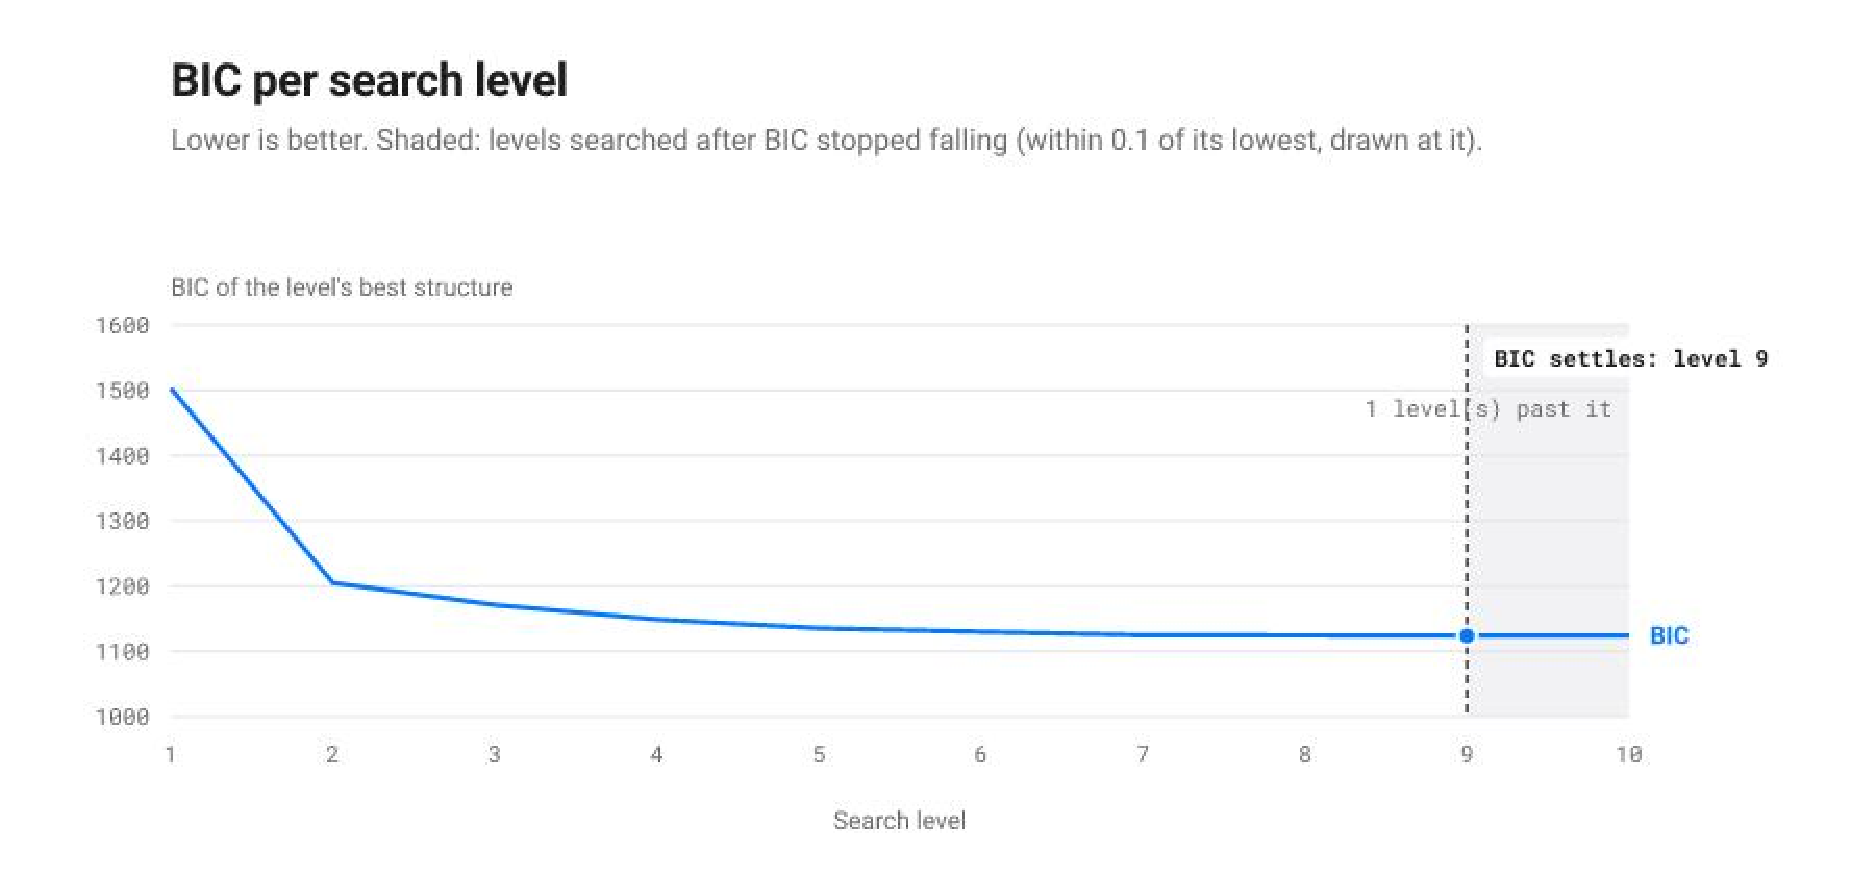
\includegraphics[keepaspectratio]{../figures/bic_airline.pdf}}
\caption{BIC per level of the published airline search. The structure
settles at level 7. The last three levels only refit it.}
\end{figure}

\begin{figure}
\centering
\pandocbounded{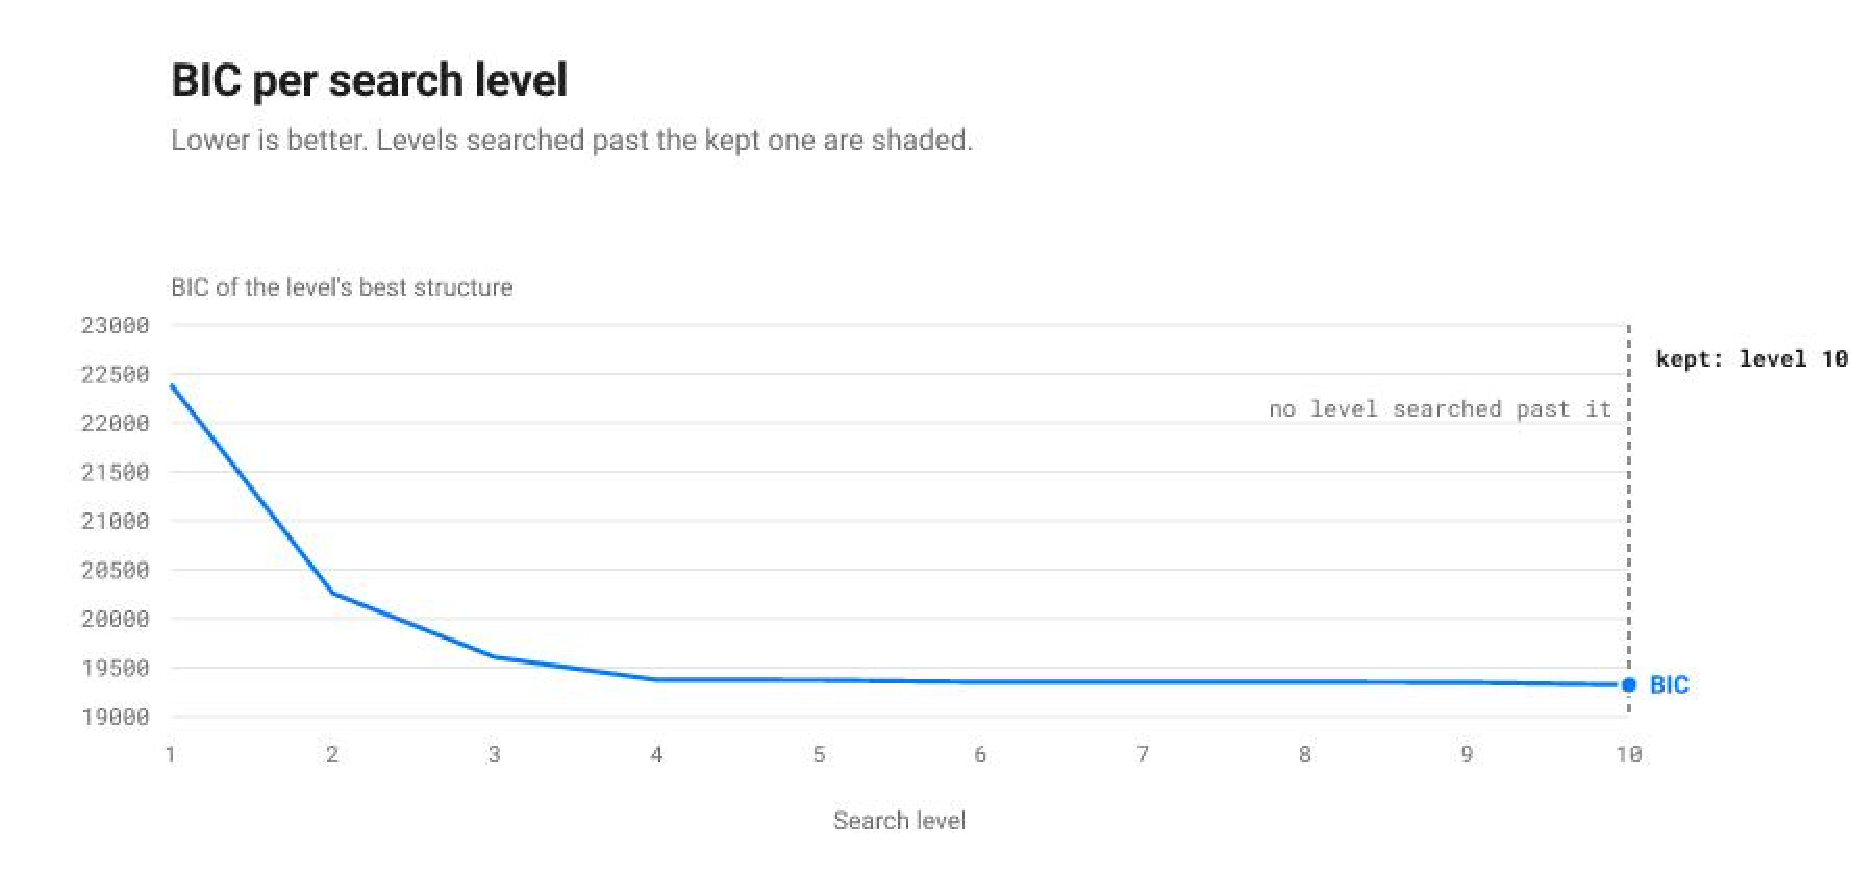
\includegraphics[keepaspectratio]{../figures/bic_internet.pdf}}
\caption{BIC per level of the published internet search. BIC stays flat
for two levels, then a structure better by 29 BIC appears at level 10.}
\end{figure}

The table supports four findings.

\begin{itemize}
\tightlist
\item
  \textbf{Ten levels are sometimes too few.} On internet, call-centre
  and gas-production, the kept structure appears at level 10, the last
  one, so the search was still changing the expression when it was cut.
  On solar it appears at level 9.
\item
  \textbf{A flat BIC is no proof of convergence.} Stopping at the first
  level without improvement would have kept a worse model on two series:
  internet by 29.2 (very strong evidence against it) and wages by 11.4.
  Two levels of patience repair wages but not internet, where the search
  stalls for two levels before finding a much better structure.
\item
  \textbf{Much of the depth goes into refitting.} On nine series the
  kept structure is found by level 8. The later levels only refit its
  parameters. On six of them that refit is worth 5.5 BIC or less. It is
  worth 9.3 on sulphuric, 35.5 on mauna and 44.2 on unemployment. On
  those three, the random restarts find better parameters for an
  expression the search already has. Depth buys optimisation as well as
  structure.
\item
  \textbf{The last level is not always the best.} On temperature, radio,
  unemployment and births, the kept model comes from an earlier level.
  The later levels, restarted from random initialisations, fitted no
  better.
\end{itemize}

The evidence for the kept structure against its best rival is very
strong on five series, strong on two and positive on five. On
call-centre it is barely worth mentioning (1.9): two expressions explain
the data about equally well. Read that report as one of the two.

The examples in \texttt{examples/} therefore search until BIC has not
fallen by 0.1 for two levels in a row, with at most twenty levels, then
report the levels past the best one. Each report has a section ``Search
path and stopping criterion'' with the BIC curve, the table above for
its own search and these readings. When the search ran a single level,
the report says there is no curve to draw.

\subsection{How much the data prefer the kept
structure}\label{how-much-the-data-prefer-the-kept-structure}

A gap in BIC is hard to feel. How much more likely is the kept structure
than its rival when the gap is 1.9? Or 4.6?

Half the BIC approximates minus the log of the marginal likelihood. So
\(\exp(-\mathrm{BIC}/2)\) is, up to a constant shared by all structures,
how likely each structure makes the data. Give every structure the same
prior weight and normalise over the structures the search met, each with
its lowest BIC. Each structure then has a posterior weight. The Bayesian
machine scientist \autocite{guimera2020bms} weighs its arithmetic
expressions the same way.

The order of magnitude checks out by hand. A gap of 4.6 gives a ratio of
\(\exp(-2.3) \approx 0.10\), so the rival is ten times less likely than
the kept structure. The sales example of \texttt{EXAMPLES.md} shows
exactly that, with weights of 0.899 for \texttt{Lin\ +\ WN\ +\ Per} and
0.092 for \texttt{Lin\ +\ WN\ +\ Per\ x\ SE}. On the published
call-centre search, the gap of 1.9 gives 0.713 to the kept structure and
0.281 to the next.

Each report now states these two weights in one sentence and reads them
on three levels, according to the rival's weight:

\begin{itemize}
\tightlist
\item
  above 0.25, the data barely tell the two structures apart
  (call-centre)
\item
  between 0.05 and 0.25, the data favour the kept one without ruling the
  next out (sales)
\item
  below 0.05, the kept structure takes almost all the weight
\end{itemize}

The section ``Search path and stopping criterion'' adds the table of
weights for every structure met with a weight of at least 0.001.

AutoGP needs a different picture, because it has no search levels and so
no BIC curve. Its summary report draws one horizontal stem per structure
kept by the posterior. The stem is as long as that structure's BIC above
the lowest and carries the structure's posterior weight as a label. A
sentence then says whether BIC agrees with the posterior on which
structure comes first. With a single structure, the summary says there
is no BIC to compare.

\section{Limits}\label{limits}

\begin{itemize}
\tightlist
\item
  \textbf{Cost.} Exact GP inference grows with the cube of the number of
  points, so the series are binned to 1,000 points. The full airline
  search took 4.1 hours on six processes. Scalable bounds
  \autocite{kim2018scaling} and Bayesian optimisation over the grammar
  \autocite{malkomes2016bayesian,bitzer2022structural} search with fewer
  evaluations. Neither is ported.
\item
  \textbf{One input.} The search handles one time input. Multivariate
  grammars \autocite{duvenaud2011additive} and structure shared across
  series \autocite{hwang2016relational} are not ported.
\item
  \textbf{Formulas.} Without PySR, or when no short formula comes within
  1 \%, smooth components keep their covariance as their formula.
\item
  \textbf{Benchmark.} TabPFN-TS \autocite{hoo2025tabpfnts} did not run
  because of its licence. AutoGP.jl, GPy-ABCD
  \autocite{fletcher2021gpyabcd}, AutoBNN \autocite{koster2024autobnn}
  and Moirai \autocite{woo2024moirai} did not install on the benchmark
  machine.
\end{itemize}

\section{Related work not compared}\label{related-work-not-compared}

Neural kernel networks learn kernel sums and products by gradient
descent \autocite{sun2018nkn}. Spectral mixtures fix a flexible form
\autocite{wilson2013spectral}. Language models now propose kernels
\autocite{suwandi2025cake}, propose probabilistic programs
\autocite{li2024boxlm} or judge fits from plots
\autocite{lee2025multimodal}. Gallifrey reimplements AutoGP in JAX for
astronomy \autocite{boettner2025gallifrey}.
\textcite{steinruecken2019automatic} summarise the Automatic
Statistician project. The project's grammar descends from the matrix
decomposition grammar of \textcite{grosse2012compositionality}. Bayesian
symbolic regression \autocite{jin2019bsr,guimera2020bms} is the closest
arithmetic counterpart to a posterior over structures.

\printbibliography[title=References]

\end{document}
